\documentclass{article}
\usepackage[dutch]{babel}
\usepackage{graphicx}
\usepackage{float}
\usepackage{geometry}
\usepackage{fancyhdr}

\geometry{a4paper, top=3cm, bottom=3cm, left=2cm, right=2cm}

\title{Adviesrapport: Data-driven Business}
\author{Yujian Jiang, Max Jansen}
\date{July 2025}

\begin{document}

\maketitle

\begin{figure}
    \centering
    
\includegraphics[width=4cm]{prorail.png}
\end{figure}

\pagestyle{fancy}

\newpage
\tableofcontents

\newpage
\section{Inleiding}

\subsection{Achtergrond van het project}
Voor het vak DataDriven Business is ProRail naar de HU gekomen met de vraag of wij hulp kunnen bieden voor het DataLab. Het DataLab is een afdeling van ProRail, waar in grote hoeveelheden data verzameld wordt, wat daarna geanalyseerd en verwerkt wordt om verbeteringen toe te passen op het spoorwegnet. Het spoorwegnet is erg groot en er zullen altijd wel problemen opduiken van klein naar groot. Dit is voor iedereen erg vervelend. ProRail is daardoor veel bezig met het oplossen van de problemen en de kosten lopen daardoor ook op. En voor de reizigers is het ook vervelend. Die moeten omreizen en zullen zich ergeren als het herhalend optreed. Het is dus van groot belang dat problemen snel en efficiënt worden opgelost om zowel kosten te besparen als de tevredenheid van de reizigers te behouden.

\subsection{Het belang van een snelle oplossing}
Het is belangrijk dat er snel gehandeld moet worden. Daarvoor moet er wel duidelijk zijn wat de problemen zijn en hoe lang die gaan duren, zodat er vooruit gepland kan worden om de minste vertragingen op te lopen. Als er bijvoorbeeld een storing is, moeten de planners weten hoe lang het ongeveer gaat duren voordat het opgelost is, zodat ze alternatieve routes kunnen plannen of vervangend vervoer kunnen regelen. Nu is er dus gevraagd of er hulp geboden kan worden bij het verduidelijken van de problemen. Er is gevraagd of het mogelijk is om te voorspellen hoe lang een storing gaat duren zodat er op tijd en beter omheen gepland kan worden en de vertragingen zo beperkt mogelijk kunnen blijven.

\newpage
\section{Opdracht}

\subsection{Doel van de opdracht}
De opdracht die wij gekregen hebben is om uit te zoeken of het mogelijk is om te voorspellen hoe lang een storing gaat duren. Dit willen ze gaan doen door gebruik te maken van een applicatie die dit kan voorspellen. Op dit moment is de applicatie er nog niet. Die gaan wij maken. Maar voor dat we dat kunnen doen moeten wij inzicht krijgen over het gehele proces. We weten namelijk niet hoe ze bij ProRail aan het werk gaan. Ook moet de data grondig doorgenomen worden. De data moet worden geanalyseerd, opgeschoond en voorbereid voor de modellen die de voorspellingen gaan doen. Dan moet de applicatie gemaakt worden. Hoe het er uit gaat zien, welk model er gekozen word, en hoe het gebruikt gaat worden. Als laatste moet er gedocumenteerd worden. Er moet een duidelijke uitleg zijn, en alles moet gerapporteerd worden. Omdat het proces behoorlijk groot is, gaan we het verdelen in verschillende delen, wat uit eindelijk een geheel moet vormen.

\subsection{Deelopdrachten}

\subsubsection{Business Understanding}
Het eerste deel is de Business Understanding, zodat ons duidelijk wordt waar wij onze taken moeten vervullen en hoe het proces loopt. We doen namelijk een opdracht voor een extern bedrijf waar wij nergens bekend mee zijn. Ons moet duidelijk worden wat er van ons allemaal gevraagd word. We moeten weten wie de stakeholders zijn, waar onze data vandaan komt, en wat de knelpunten zijn. Maar ook hoe hun hele proces loopt, hoe het bedrijf aan het werk gaat, wat onze rol is. Pas als wij snappen hoe ProRail werkt. Kunnen wij een opdracht voor ze maken.

\subsubsection{Data}
Als het eenmaal duidelijk is wat we moeten gaan doen, is de volgende stap het begrijpen van de data. Zonder de data kunnen we namelijk geen voorspellingen maken. De data is erg ingewikkeld en ver van schoon. We hebben 58 kolommen met allemaal onduidelijke namen. Ook zijn er $\pm$ 800.000 rijen waar we mee werken, en er staan heel veel lege/verkeerde waarden in. Het is dus een zooitje. Nu is het belangrijk om te begrijpen wat alles is, wat er uit gefilterd mag worden en waar we mee doorgaan. Daarnaast moet er goed worden geanalyseerd, zodat er vervolgens drie modellen uitgewerkt kunnen worden.

\subsubsection{Modellen}
Als we eenmaal inzicht hebben in de data, kunnen we beginnen met het bouwen van modellen. Het doel hiervan is om voorspellingen te doen die het werkproces kunnen ondersteunen. We gaan meerdere modellen testen, zodat we kunnen bepalen welke het beste werkt voor onze situatie. Belangrijk is dat we goed uitleggen waarom we bepaalde keuzes maken, welke algoritmes we gebruiken, en hoe accuraat de modellen zijn. Elk model heeft zijn eigen voor- en nadelen, en moet goed geanalyseerd worden. Uiteindelijk kiezen we het model dat het meest betrouwbaar is en het beste past bij de voorspellingen die gemaakt moeten worden. Dit model wordt dan verwerkt in de applicatie.
 
\subsubsection{Applicatie}
Het belang van de opracht is een werkende applicatie. Dit gaat namelijk gebruikt worden door het personeel in de meldkamer, waar de storingen verwerkt worden. Hier komt het hele project samen. De applicatie gaat een van de gekozen modellen bevatten die de voorspelling gaat doen. Die gecreëerd is uit de analyse van de data. Maar ook omdat we inzicht hebben gecreëerd voor het bedrijf. Ook kan je alle oude data terug vinden om te kijken hoe de oude storingen waren, maar ook hoe lang het duurde voordat ze waren opgelost.

\subsubsection{Documentatie}
Om het project af te ronden is er goede documentatie nodig. Je kan wel een werkend product neer zetten maar als het niet duidelijk is hoe het gebruikt moet gaan worden kom je niet ver. Er wordt een duidelijke uitleg verwacht van hoe de applicatie gebruikt moet worden, maar ook hoe het model tot stand gekomen is. Er moet namelijk wel een goede reden zijn om geld en tijd te investeren in deze applicatie.
 
\newpage
\section{Business Understanding}

\subsection{Process}
De eerste stap in het project, is het in kaart brengen van het probleem, en de oplossing waar we naartoe moeten werken. Om het probleem in kaar te brengen zijn wij druk bezig geweest met de mensen van ProRail om alles in kaart te brengen. Het proces begint wanneer iemand (de melder) een probleem opmerkt en contact opneemt met de meldkamer. De meldkamer zoekt vervolgens een aannemer die beschikbaar is en belt deze op. Zodra de aannemer onderweg is, maakt hij een prognose van het probleem. Op basis daarvan wordt bepaald of de treindienstregeling moet worden aangepast. Als dat zo is, wordt de planner op de hoogte gebracht. De aannemer komt aan op locatie en lost het probleem op. Tijdens dit hele proces worden belangrijke gegevens vastgelegd, zoals de oorzaak, locatie en duur van de storing. Zodra het probleem is opgelost, communiceert de meldkamer dit terug naar de betrokken partijen. De aannemer vertrekt en als alles in orde is, worden de treinen weer hervat. Dit hele proces is belangrijk om te snappen, omdat wij hierdoor weten op welk moment er welke data beschikbaar is, en waar onze applicatie het meest van waarde kan zijn.

\begin{figure}[H]
    \centering
    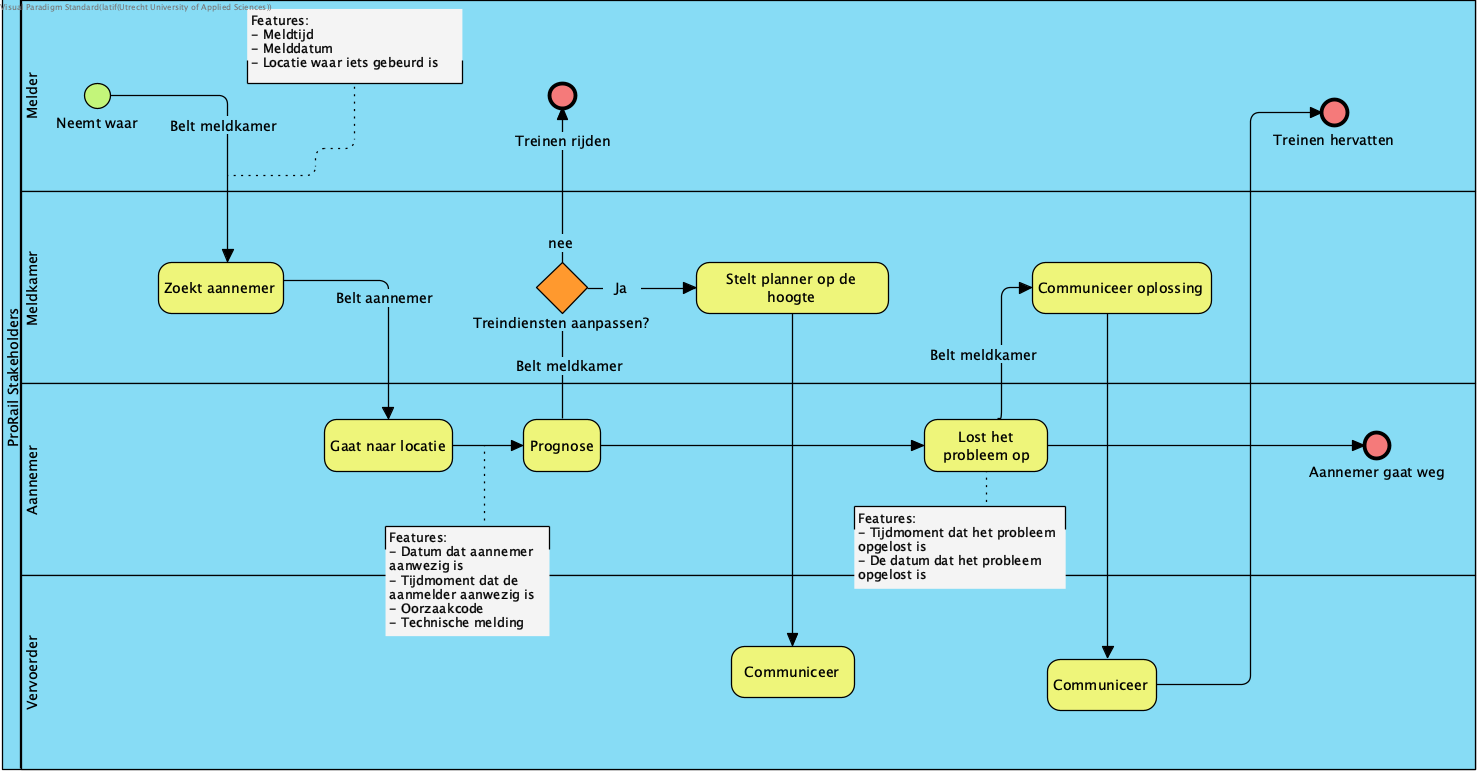
\includegraphics[width=10cm]{bpmn.png}
    \caption{BPMN (Business Process Model and Notation)}
\end{figure}

\subsection{Stakeholders}
Tijdens het project hebben we gekeken naar wie er allemaal betrokken zijn bij het proces rondom een storing, en wie er dus belang hebben bij een betere manier van voorspellen. Deze belanghebbenden (oftewel stakeholders) zijn de mensen of partijen die direct of indirect geraakt worden door een storing, en dus ook baat hebben bij een goede oplossing. Omdat we te maken hebben met een groot proces met meerdere stappen en afdelingen, zijn er best veel belanghebbenden.

\begin{itemize}
    \item \textbf{Meldkamer van ProRail:} Hier begint het hele proces. De meldkamer ontvangt de melding van de storing en moet direct actie ondernemen. Ze schakelen een aannemer in en houden contact met alle betrokkenen. Voor hen is het handig om zo snel mogelijk te weten hoe lang iets ongeveer gaat duren, zodat ze kunnen schakelen.

    \item \textbf{Planners van ProRail:} Zodra een storing invloed heeft op het spoor, moeten planners beslissen of er een aangepaste dienstregeling nodig is. Hoe beter ze weten hoe lang een storing gaat duren, hoe beter ze dat kunnen inschatten. Zonder goede informatie is het vaak gokken, en dat zorgt voor extra overlast.

    \item \textbf{Aannemers:} De mensen die daadwerkelijk naar de storing toegaan en het probleem oplossen. Zij geven belangrijke informatie door, zoals de oorzaak en wanneer ze ter plekke zijn. Deze info gebruiken wij in onze modellen om te voorspellen hoe lang het nog gaat duren.

    \item \textbf{Vervoerders:} Als een storing impact heeft op het treinverkeer, zijn de vervoerders daar de dupe van. Zij moeten hun treinen en personeel opnieuw inplannen en zorgen dat reizigers weten waar ze aan toe zijn. Hoe sneller zij weten wat de impact is, hoe sneller ze kunnen schakelen.

    \item \textbf{Reizigers:} De mensen die elke dag met de trein reizen. Zij hebben natuurlijk geen invloed op het proces, maar ze merken de gevolgen wel direct. Door betere voorspellingen kunnen we de vertraging voor hen zoveel mogelijk beperken en beter communiceren wat er aan de hand is.

    \item \textbf{DataLab van ProRail:} Het DataLab is de afdeling binnen ProRail die zich bezighoudt met innovatie en data. Zij hebben ons gevraagd om dit project op te pakken. Ze willen weten of machine learning hierbij kan helpen, en of onze aanpak in de praktijk toegevoegde waarde biedt.

    \item \textbf{Ons projectteam (HU-studenten):} Tot slot zijn wij zelf ook belanghebbenden. Voor ons is het belangrijk dat het project duidelijk afgebakend is, dat de data bruikbaar is, en dat we goede feedback krijgen. Alleen dan kunnen wij iets maken wat echt gebruikt gaat worden.
\end{itemize}

\subsection{Knelpunten}
Tijdens het project kwamen we verschillende knelpunten tegen, zowel in het proces als in de data. Deze punten zorgen ervoor dat het moeilijk is om direct een goed werkend model of systeem te maken. Hieronder de belangrijkste knelpunten die we zijn tegengekomen:

\begin{itemize}
  \item \textbf{Inzicht in het proces:} In het begin was het onduidelijk hoe het proces precies verliep binnen ProRail. Omdat we extern zijn, wisten we niet wat er allemaal gebeurt vanaf het moment dat een storing gemeld wordt tot aan de oplossing. Daardoor was het lastig om te bepalen waar onze applicatie echt waarde kon toevoegen.
  \item \textbf{Datakwaliteit:} De data waar we mee werken is allesbehalve perfect. Er zitten veel lege velden in, foutieve of inconsistente waarden, en soms ontbreekt essentiële informatie. Dit maakt het moeilijk om betrouwbare voorspellingen te doen. Ook is de data erg technisch en soms lastig te interpreteren.
  \item \textbf{Tijdstip van datatoegang:} Niet alle informatie is meteen beschikbaar wanneer een storing net gemeld is. Sommige data komt pas later in het proces binnen, bijvoorbeeld als de aannemer ter plekke is. Daardoor kunnen we niet altijd meteen een goede voorspelling doen.
  \item \textbf{Complexiteit van het probleem:} Het voorspellen van de duur van een storing is lastig, omdat elke storing anders is. De ene keer is het een kapotte bovenleiding, de andere keer een wisselstoring. Er zijn veel factoren die invloed hebben, en die zijn lang niet altijd duidelijk of meetbaar.
  \item \textbf{Gebrek aan standaardisatie:} Veel waarden in de data zijn handmatig ingevoerd en worden niet altijd op dezelfde manier geregistreerd. Dit zorgt voor ruis in de data en bemoeilijkt het trainen van een goed model.
\end{itemize}

\newpage
\section{Data}

\subsection{Waar we mee werken}
Nu we weten hoe het hele proces verloopt, kunnen we ons gaan richten op mischien wel het belangrijkste deel van het project: de data. Op basis van de data gaan de voorspellingen gemaakt worden namelijk. En als we niet goed begrijpen hoe de data werkt, kunnen we geen goede modellen maken. Daarom zijn wij grondig onderzoek gaan doen waar we mee te werk gaan. 

Het is dus ook belangrijk om te weten hoe de data in elkaar zit en wat we gaan gebruiken. Door het proces goed te begrijpen, kunnen we bepalen op welk moment in de workflow onze voorspellingen het meest nuttig zijn. Bijvoorbeeld, zodra een storing gemeld wordt, is er nog weinig informatie beschikbaar. Maar wanneer de aannemer ter plekke is, hebben we meer data om een nauwkeurige voorspelling te maken.

\subsection{Het Onderzoek}
JUPYTER NOTEBOOK NALOPEN

Daarna zijn we ons gaan focussen op de data. Dit is een van de belangrijkste onderdelen aangezien we moeten weten waar we mee werken. Er moet zekerheid zijn over de data of alles wel juist is. Er staan vaak namelijk verkeerde en/of zelfs lege plekken in de data. Als eerste zijn we gaan onderzoeken wat er allemaal in de data zit.

\subsection{Opschonen van de data}
JUPYTER NOTEBOOK NALOPEN

De volgende stap is om te zorgen dat er meer duidelijkheid komt over wat de data inhoudt. Het is opgevallen dat er inconsistenties zijn in de data, zoals ontbrekende waarden en foutieve invoer. We moeten deze issues oplossen om accurate voorspellingen te kunnen maken. We hebben daarom de data opgeschoond door ontbrekende waarden te vullen of te verwijderen waar nodig, en fouten te corrigeren. Bijvoorbeeld, als er een tijd ontbreekt, kunnen we die niet gebruiken in ons model. Ook hebben we ervoor gezorgd dat alle data in het juiste formaat staat, zoals het omzetten van datums naar numerieke waarden die het model kan begrijpen.

\subsection{Gekozen features}
Op het eerste oog zijn wij breedschalig gaan kijken welke kolommen wij willen gebruiken. Uiteindelijk hebben we besloten om de volgende kolommen te gebruiken:
\begin{itemize}
  \item \textbf{stm\_sap\_melddatum}: De datum van de melding.
  \item \textbf{stm\_sap\_meldtijd}: De tijd van de melding.
  \item \textbf{stm\_aanntplj\_tijd}: De tijd dat de aannemer ter plaatsen in. 
  \item \textbf{stm\_progfh\_in\_duur}: De prognose van de functie hersteltijd.
  \item \textbf{stm\_prioriteit}: De prioriteit van de storing.
  \item \textbf{stm\_oorz\_code}: De oorzaak code vaar de storing in valt.
  \item \textbf{stm\_contractgeb\_mld}: Het contractgebied van de melding.
  \item \textbf{stm\_techn\_mld}: De techniekveld van de melding.
\end{itemize}
Deze kolommen hebben we gekozen omdat ze het meest relevant zijn voor het voorspellen van de hersteltijd. Ons target, oftewel wat we willen voorspellen, is targetherstel. Dit is de tijd die het duurt vanaf het moment dat de aannemer aanwezig is tot het moment dat het incident verholpen is.

\subsection{Voorspel Target}
Lorem Ipsum

\newpage
\section{Modellen}

\subsection{Lineaire Regressie}
Lorem Ipsum

\subsection{Decision Tree}
Lorem Ipsum

\subsection{Random Forest}
Lorem Ipsum

\section{Resultaten van de modellen}
Lorem Ispum

\newpage
\section{Applicatie}

\subsection{Ontwerp van de applicatie}
Het model waarin de voorspelling wordt gemaakt is erg ingewikkeld en vereist technische kennis. Daarom is er een applicatie gemaakt waarin je op een gebruiksvriendelijke manier hetzelfde resultaat kunt behalen. Omdat een goede applicatie maken veel werk kost, zijn wij als eerste visuele en interactieve ontwerpen gaan maken om te laten zien hoe de applicatie eruit gaat zien. We hebben wireframes en prototypes gemaakt om het ontwerp te testen. De applicatie moet intuïtief zijn, zodat gebruikers zonder technische achtergrond er mee kunnen werken.

\subsection{Implementatie en veiligheid}
Na dit getest te laten hebben zijn wij begonnen met het uitwerken van de applicatie, die vervolgens op het web geplaatst wordt zodat de betrokkenen er altijd bij kunnen. Omdat de applicatie online staat hebben wij ons ook gefocust op de veiligheid, en is het dus niet toegankelijk voor iedereen. Er is een systeem gebouwd dat ervoor zorgt dat alleen de mensen met een account er toegang tot hebben. We hebben ook gebruik gemaakt van beveiligde verbindingen (SSL) om de data te beschermen. De applicatie bevat ook een helpsectie, zodat gebruikers snel antwoord kunnen vinden op hun vragen.

\newpage
\section{Conclusie}
Door het combineren van data-analyse en machine learning is het mogelijk om nauwkeurige voorspellingen te doen over de hersteltijden van storingen. Dit stelt ProRail in staat om beter te plannen en de impact op reizigers te minimaliseren. De ontwikkelde applicatie maakt het eenvoudig voor gebruikers om deze voorspellingen te raadplegen en draagt bij aan een efficiënter spoorwegsysteem. Het decision tree model heeft bewezen het meest effectief te zijn en kan in de toekomst verder verbeterd worden met meer data.

\end{document}
